% This version of CVPR template is provided by Ming-Ming Cheng.
% Please leave an issue if you found a bug:
% https://github.com/MCG-NKU/CVPR_Template.

% \documentclass[review]{cvpr}
\documentclass[final]{cvpr}

\usepackage{times}
\usepackage{epsfig}
\usepackage{graphicx}
\usepackage{amsmath}
\usepackage{amssymb}

% Include other packages here, before hyperref.

% If you comment hyperref and then uncomment it, you should delete
% egpaper.aux before re-running latex.  (Or just hit 'q' on the first latex
% run, let it finish, and you should be clear).
\usepackage[pagebackref=true,breaklinks=true,colorlinks,bookmarks=false]{hyperref}


\def\cvprPaperID{****} % *** Enter the CVPR Paper ID here
\def\confYear{CVPR 2021}
%\setcounter{page}{4321} % For final version only


\begin{document}

%%%%%%%%% TITLE
\title{Automated Camera Stabilization and Calibration \\for Intelligent Transportation Systems}

\author{Marcel Bruckner\\
% Informatics 6 - Chair of Robotics, Artificial Intelligence and Real-time Systems\\
% TUM Department of Informatics\\
Technische Universität München\\
Boltzmannstraße 15, 85748 Garching\\
{\tt\small marcel.bruckner@tum.de}
}

\maketitle

% !TEX root=./report.tex

\newcommand{\Providentia}{\emph{\href{https://innovation-mobility.com/}{Providentia++}} project \cite{kraemmer2020providentia}} 
\newcommand{\TAADBW}{\emph{Test Area Autonomous Driving Baden-Württemberg} \cite{fleck2018towards}} 
\newcommand{\ITS}{Intelligent Transportation System}
\newcommand{\AD}{Autonomous Driving}
\newcommand{\HDmaps}{HD maps~(\ref{sec:hd_maps})}
\newcommand{\Sc}{static scene (\ref{sec:dynamic_foreground_static_scene})}
\newcommand{\DigitalTwin}{Digital~Twin~(\ref{sec:digital_twin})}
\newcommand{\OD}{OpenDRIVE}

\newcommand{\camsn}[1]{S{#1}0 Near}
\newcommand{\camsf}[1]{S{#1}0 Far}

\newcommand{\hr}{\noindent\rule{\linewidth}{0.4pt}}


\providecommand{\keywords}[1]
{
  \small	
  \textbf{\textit{Keywords---}} #1
}

\newcommand\blankpage{%
    \null
    \thispagestyle{empty}%
    \addtocounter{page}{-1}%
    \newpage}

%%%%%%%%% ABSTRACT
%!TEX root = ../report.tex
\begin{abstract}

In the emerging field of Intelligent Transportation Systems one main challenge is the fusion of different sensor types.
To fuse the measurements correctly each sensor needs to be free from noise and calibrated accurately.

In this work we focus on two problems resulting from environmental influences on RGB cameras within the Providentia++~project.

First we propose an online vision-based framework to remove jitter from shaky camera streams to dynamically stabilize the video feed.
We show that our approach based on visual features and an image space homographic transformation gives good stabilization results regarding the optical flow in the image. 
By exemplary tracking objects and measuring their travelled pixel distance we show a substantial decrease of the jittery image motion. 

Second we propose an online Bundle Adjustment formulation based on the reprojection-error to statically calibrate RBG-only cameras \wrt{} a high definition map and to mitigate drift of the intrinsic and extrinsic camera parameters over time.
By relaxing the minimization problem using a 1D-approximation of road signs we achieve high accuracy in the calibration of the cameras.
We show the minimal number of needed correspondences between the video stream and the map, the structure they have to exceed and give a lower bound on the remaining calibration error. 

\end{abstract}


\keywords{
    Intelligent Transportation Systems,
    Computer Vision,
    Video Stabilization,
    Feature Detection,
    Feature Matching,
    Camera Calibration,
    Bundle Adjustment,
    Reprojection-error,
    Optimization,
    OpenDRIVE
}


%%%%%%%%% BODY TEXT
% !TEX root=./report.tex

\section{Introduction}

Within the \Providentia{}, a section of the highway A9 between Munich and Nuremberg was converted to a testing site for autonomous driving. 
As part of this, a large sensor network system has been set up along the highway to allow monitoring and steering of traffic as well as to improve the coordination between autonomous and traditional cars. 
The primary task of the intelligent transportation system (ITS) is to create a digital traffic twin that accurately represents the physical road situation in real-time. 
Based on this digital twin, the smart infrastructure can provide a far-reaching and comprehensive view to the drivers and autonomous cars in order to improve their situational awareness within the current traffic environment.

A key challenge of ITS lies in the reliable and accurate calibration of the different sensors.
The calibration is especially challenging when the sensor is subject to real-life disturbances like vibration of its mounting pole caused by wind or displacements due to temperature expansion.
In this work we focus on removing the noise introduced by the disturbances and its implications for the vision system built upon the cameras mounted to gantry bridges.

We propose two computer vision based approaches to tackle the real-life disturbances and to remove noise from the system.
The solved problems can be roughly grouped into problems concerning the dynamic stabilization of the video feed and the static calibration of the camera setup.

\paragraph{Dynamic Stabilization}
The cameras are constantly exposed to wind and vibrations from passing vehicles.
These influences propagate into the video stream and result in jittery motion of the images.
We propose a pipeline to counteract the shaky motions of the cameras using a digital image stabilization approach.
The approach is based on visual image features that are matched between the current and a stable reference frame. 
The feature matching is used to minimize the reprojection-error between the frames and results in a homographic transformation.
We use the transformation to align the static backgrounds of the frames, thus mitigating the real-world motions of the camera in the image space.

\paragraph{Static Calibration}
We track and predict the real world location of the vehicles in the test to pass this information to the drivers and autonomous vehicles. 
To accurately predict the locations the system needs to be calibrated precisely towards a global reference frame. 
This is a time consuming process that often has to be done by hand. 
The cameras translational, rotational and intrinsic parameters decalibrate over time due to environmental influences on the mounting constructions and gantry bridges as well as from the natural wear of the materials.

Within the project high definition maps (HD maps) of the enclosed environment are used extensively. 
These HD maps offer the approximations of the real-world positions of the highway lanes, the gantry bridges, objects like poles and permanent delineators and traffic signals like speed limits or exit markers.
We use this spatial information and a mapping from the objects to pixels in the video frame to solve a Bundle Adjustment (BA) problem by minimizing the reprojection-error.
We jointly optimize for the cameras intrinsic and extrinsic parameters as well as the real-world locations to recover the camera poses form the observations.

\paragraph{Code Repositories}
The code for the dynamic stabilization, static calibration and object position retrieval from the HD maps are accessible via two GitHub repositories: \url{https://github.com/Brucknem/GuidedResearch} and \url{https://github.com/Brucknem/OpenDRIVE}.


% % !TEX root=./report.tex

\section{Terms and Definitions}
This section provides explanations of extensively used terms and definitions. 

\subsection{Digital Twin}
\label{sec:digital_twin}

\subsection{Dynamic foreground and static scene}
\label{sec:dynamic_foreground_static_scene}
We group parts of the world seen by the cameras into the two groups of dynamic foreground and static scene.
Dynamic foreground describes all pixels that represent objects that are meant to be moving, \eg{} vehicles on the roads.
On the other hand the static scene are all pixels that are not dynamic foreground, \eg{} the road, guardrails or bridges.

\subsection{Parametric cubic polynomial}
To calculate a parametric cubic polynomial the following equation is used.
\begin{equation}
    \begin{split}
        para(U, s) &= para(U_a, U_b, U_c, U_d, s) \\ &= U_a + U_b * s + U_c * s^2 + U_d * s^3
    \end{split}
\end{equation}
% \section{Related Work}
There are many ITS projects emerging recently  \cite{koster2017testfeld,arnold2020cooperative,arnoldCooperativePerception,agrawal2008censure}. 
They propose novel approaches to the detection, tracking and traffic prediction problems that arise with the goal to provide additional environment information to human drivers and autonomous vehicles.
Erdelean \etal{} \cite{erdelean2019catalogue} give a detailed overview over the existing projects up to the year 2019.

In the \TAADBW{} (TAADBW) project multiple optical camera sensors are attached to large poles with overlapping fields of view.
They calibrate their cameras relative to a high-precision map and assume the calibration and the intrinsic camera parameters to be static during runtime. 
The team relies on a manual a-priori selection of visual landmarks and perform calibration at system startup.  
The team of the TAADBW estimate the extrinsic calibration with exact world position from the map by minimizing the squared distances between the visible landmarks and the respective projected objects.
The large overlaps in the fields of view in their setup allow a global optimization strategy. 
This is not feasible in our project due to the small overlaps in the fields of view between the cameras \cite{kraemmer2020providentia} and associating pixels within the multi-view setup is an inherently hard problem. 

Müller \etal{} \cite{laciMueller} present an approach based on a cooperative intelligent vehicle.
The vehicle moves through the scene and passes cooperative awareness messages containing positional information from the vehicle to the infrastructure. 
This removes the need for overlapping fields of view completely and enables a fully automated and sensor-independent registration.
The team calibrates a multitude of different sensor types to the world frame and recovers their extrinsic parameters. 

Calibration between cameras and radar sensors has been solved previously by Schöller \etal{} within the \Providentia{}.

An overview over the general structure of Bundle Adjustment problems as used in \autoref{sec:static_calibration_approach} is given by Triggs \etal{} in \cite{triggs10.1007/3-540-44480-7_21}.
% None of the teams - to the best of our knowledge - provide in depth public information about their camera stabilization and calibration approaches.
% % !TEX root=./report.tex

\section{Approach}
In this paper we propose two algorithms to solve distinct problems that arise from the real-world disturbances that act upon the \ITS{}.

\subsection{Dynamic stabilization}
The gantry bridges to which the cameras are mounted are prone to environmental influences. 
These influences include, but not exclusively, wind and vibrations from passing vehicles.
These external influences bring the cameras into a swinging state which introduces jittery motion in the video feeds.

Although the displacements of the camera only span a small range around its resting position, the influences in on the images amplify by the huge distances the cameras overview.

To mitigate the noise added by the jittery motion we propose the pipeline displayed in \autoref{fig:dynamic_stabilization_algorithm}.

\begin{figure}[t]
  \begin{center}
  % \fbox{\rule{0pt}{2in} \rule{0.9\linewidth}{0pt}}
     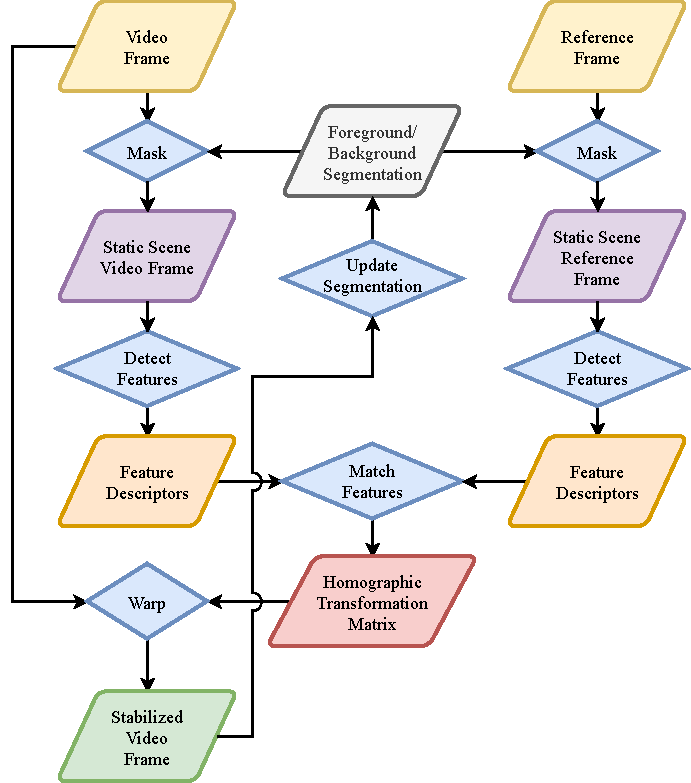
\includegraphics[width=0.8\linewidth]{diagrams/DynamicStabilization.pdf}
  \end{center}
     \caption{}
  \label{fig:dynamic_stabilization_algorithm}
  \end{figure}

\paragraph{Frame retrieval}
The first step in the algorithm is to retrieve the current frame from the camera.

\paragraph{Removing dynamic foreground scene}
We only want to find features on the non-moving \Sc{} objects, \eg{} the road, poles, guardrails and bridges. 
As these features are expected to not move between frames, aligning these during image warping ensures that the scene stays static.
Moving vehicles are thus excluded from the detection and do not contribute in the algorithm.

Hence, we mask the current video frame and the stable reference frame using a background segmentation based on
the \emph{Improved Adaptive Gaussian Mixture Model for Background Subtraction} proposed by Zoran Zivkovic \etal{} \cite{zivkovic10.5555/1018428.1020644,zivkovic10.1016/j.patrec.2005.11.005,opencv_library}.

Additionally it speeds up the algorithm. 

Maybe append more about warmup for MOG2.

\paragraph{Feature detection}
We are looking for specific patterns or specific features which are unique, can be easily tracked and can be easily compared. (Taken from OpenCV)

Hence, on the \Sc{} of the video frame and reference frame we perform feature
detection to retrieve the descriptors and pixel locations of prominent image
parts.

There exists many different implementations of feature detectors and descriptors
as described by Kumar \etal{} \cite{kumar2014survey}. We mainly focus on the
implementations of SIFT \cite{lowe10.1023/B:VISI.0000029664.99615.94}, SURF
\cite{bay10.1007/11744023_32} and ORB \cite{rublee6126544} feature detectors and
descriptors, Fast \cite{Ghahremani_2021} feature detector with FREAK \cite{alahi6247715} feature
descriptors and Star \cite{agrawal2008censure} feature detector with BRIEF \cite{calonder10.5555/1888089.1888148} feature descriptors coming from the OpenCV library \cite{opencv_library}. 

\paragraph{Feature matching}
Feature matching compares the features of one frame to the features of the other frame.
A match is reported if the feature descriptors of two compared features surpass a specific dynamic
threshold \cite{lowe10.1023/B:VISI.0000029664.99615.94} regarding some feature
dependent metric \cite{kumar2014survey}.
These feature matches establish a spatial relationship in pixel space between the two frames.

\paragraph{Frame warping}



\subsection{Static calibration}
\begin{itemize}
  \item HD map based approach
  \item Optimization algorithm, reprojection error between map and video 
  \item Landmark extraction, mapping, pose estimation
  \item Watersheder for pixel marking
\end{itemize}
% \section{Evaluation}
% % !TEX root=./report.tex

\section{Future Work}
The project leaves us with the opportunity to continue the research in multiple directions.

\subsection{Varying Weather and Lighting Conditions}
We tested and evaluated the implementations on recordings with good weather and lighting conditions, thus a next step is to test the implementations in bad weather and lighting conditions, \eg by night, rain and snow.
From out current perspective the feature based dynamic stabilization approach will suffer in performance as the homography estimation depend on features in the image space. 
By night and if the static background is occluded the stabilization pipeline will fail, although in these cases the complete RGB image will be unusable at all.

We implemented the solver for the BA problem to include human interaction when mapping from PDs to pixels.
The mapping will be harder in bad weather and lighting conditions based on the worse visibility of the landmarks.
We propose an automatic mapping scheme in \Cref{sec:auto_mapping_landmarks}.
This scheme will be affected by changing weather and lighting conditions as the detection of new landmarks is also based on the visibility of landmarks.

%%%%%%%%%%%%%%%%%%%%%%%%%%%%%%%%%%%%%%%%%%%%%%%%%%%%%%%%%%%%%%%%%%%%%%%%%%%%%%%%%%%%%%%%%%%%%%%%%%%%%%%%%%%%%%%%%%%%
%%%%%%%%%%%%%%%%%%%%%%%%%%%%%%%%%%%%%%%%%%%%%%%%%%%%%%%%%%%%%%%%%%%%%%%%%%%%%%%%%%%%%%%%%%%%%%%%%%%%%%%%%%%%%%%%%%%%
%%%%%%%%%%%%%%%%%%%%%%%%%%%%%%%%%%%%%%%%%%%%%%%%%%%%%%%%%%%%%%%%%%%%%%%%%%%%%%%%%%%%%%%%%%%%%%%%%%%%%%%%%%%%%%%%%%%%

\subsection{Dynamic Stabilization}
We present two major improvements that can be done to extend the presented dynamic stabilization approach.

\subsubsection{Warp Field Stabilization Based on Optical Flow}
We use the optical flow to measure the performance of the stabilizers as described in  \Cref{sec:evaluation_dynamic_stabilization_optical_flow}.
The optical flow is a 2D vector field where each vector is a displacement vector showing the movement of pixels between frames caused by movement of the objects or cameras.
The image can be stabilized using the inverse vector field that also minimizes the reprojection error between frames.

\subsubsection{Deep Learning Based Dynamic Stabilization}
Based on the ongoing success of deep learning approaches in computer vision, especially of convolutional neural networks (CNN), a self-learning stabilization procedure might be developed.
The CNN expects the current input and reference frame and outputs the homographic transformation or the warped frame. 
This might speed up the pipeline and inherently adds a measure for the uncertainty of the results by modelling the probability of the homographic transformation.
This approach can be used to fuse the feature detection, matching and warping steps into one joint step that is learned by the CNN from labeled data.

%%%%%%%%%%%%%%%%%%%%%%%%%%%%%%%%%%%%%%%%%%%%%%%%%%%%%%%%%%%%%%%%%%%%%%%%%%%%%%%%%%%%%%%%%%%%%%%%%%%%%%%%%%%%%%%%%%%%
%%%%%%%%%%%%%%%%%%%%%%%%%%%%%%%%%%%%%%%%%%%%%%%%%%%%%%%%%%%%%%%%%%%%%%%%%%%%%%%%%%%%%%%%%%%%%%%%%%%%%%%%%%%%%%%%%%%%
%%%%%%%%%%%%%%%%%%%%%%%%%%%%%%%%%%%%%%%%%%%%%%%%%%%%%%%%%%%%%%%%%%%%%%%%%%%%%%%%%%%%%%%%%%%%%%%%%%%%%%%%%%%%%%%%%%%%

\subsection{Static Calibration}
We present two major improvements that can be done to extend the presented static calibration approach.

\subsubsection{Robustness Against Outliers}
BA problems are inherently prone to outliers, as they greatly impact the shape of the reprojection-error loss landscape. 
To use the presented system in practice a RANSAC \cite{fischler1981random} or similar sample consensus based approach needs to be implemented.
By evaluating the calibration multiple times with different subsets of correspondences a stable sample consensus can be found in asymptotically all runs.
This will greatly impact the robustness of the calibration procedure against outliers, as they can be filtered out automatically by the algorithm.  


\subsubsection{Fully Automatic Static Calibration}
\label{sec:auto_mapping_landmarks}
We establish the mapping of the correspondences by hand, thus a human has to look up the ids of the landmarks in the HD maps and assign them to their respective pixels.
After an initial calibration that requires human interaction, an image region based approach might be used to automate this mapping.
One can project the known base origin points of the objects from the HD maps into the current frame.
Starting from the projected pixel locations one could search in a defined enclosing region to find pixels that clearly correspond to the objects by applying template, color or gradient matching approaches.
The automatic detection of landmarks enables the system to perform fully automatic static self calibration.

\subsubsection{Machine Learning Based Bundle Adjustment}
Aravkin \etal \cite{students_t_bundle_adjustment} have shown that the BA problem can be modelled on top of a Student's-t distribution. 
The resulting statistical machine learning approach for the BA can be used to jointly estimate the camera parameters and world positions of objects, while at the same time being robust against outliers.
  
\subsubsection{New High Definition Map}
The newer OpenDRIVE standard also provides the possibility to include lane markings.
These lane markings are easily detectable and can be used for the calibration procedure in conjunction with the object landmarks.
This would greatly simplify the automatic detection and mapping procedures as described in \Cref{sec:auto_mapping_landmarks} as they are spatially more extend and thus easier to detect.
Furthermore, the lane markings are always white or yellow which simplifies the detection.
As shown in \Cref{sec:static_calibration_expectable_error} the static calibration is more precise the closer the correspondences are to the cameras. 
As there exists far more lane markings than objects, and with the markings being evenly distributed over the road the static calibration would benefit from this additional information.
% % !TEX root=./report.tex

\section{Conclusion}

In this paper we proposed two main improvements on the vision based tracking system used in the \Providentia{}.

We first presented a pipeline to dynamically stabilize jittery motion in the video streams of RGB cameras mounted to gantry bridges along a highway.
We applied a homographic transformation in image space based on the matching of visual features between the current and a stable reference frame.
We have shown that the stabilization substantially (up to $99.8\%$) improves the stability of the frames regarding the remaining mean pixel displacement.
By tracking vehicles through the video sequence we have shown that the remaining length of the pixels path after stabilization is lowered by up to $57\%$ compared to the not stabilized one and thus the jittery motion of the camera is compensated significantly after stabilization.
Finally, we have shown that the dynamic stabilization pipeline is easily realtime capable with at least $50$ processed frames per second.

We secondly presented the formulation of a single camera RGB-only Bundle Adjustment problem that is minimized using the reprojection-error to statically calibrate the camera setup to the reference system.
We recover the cameras pose by jointly optimizing for the cameras intrinsic and extrinsic parameters as well as the real world position of viewed correspondences to a high definition map.
We checked our results for the absence of systematic errors, gave a lower bound on the number of correspondences needed for convergence and the structure the correspondences have to exceed.
We evaluated the expectable error after pose estimation that arises from measurement uncertainties and imprecisions in the HD map and have shown that the deviations among the minima found by the optimization strategy are neglectable.


{\small
\bibliographystyle{ieee_fullname}
\bibliography{egbib}
}

\end{document}
